\begin{problema}
\mbox{}
    \begin{enumerate}
        \item 
            Ejecute y explique la funci\'on del siguiente c\'odigo en Octave. Comente qu\'e 
            teoremas del curso (y del curso de probabilidad) son importantes para interpretar 
            la figura.
            \tiny
            \texttt
            {
                \lstinputlisting[caption=]{tarea3/problema3_4/polya2.R}
            }
            \normalsize
            (Conmigo se negó a brincar de linea. Tuve que hacerlo diminuto para que apareciera el código completo.)\par\null
        \item 
            Ejecute y explique la funci\'on del siguiente c\'odigo en Octave. 
            Incluya una gr\'afica en la que la longitud de la variable k sea mayor a 1000. 
            (Puede modificar el programa...) En la gr\'afica observara un esbozo de la 
            trayectoria de un proceso de ramificaci\'on continuo (en una escala distinta...).
            \texttt{
                \lstinputlisting[caption=]{tarea3/problema3_4/binaryGW.R}
            }
    \end{enumerate}
\end{problema}

\afterstatement\par\null

\begin{center}
    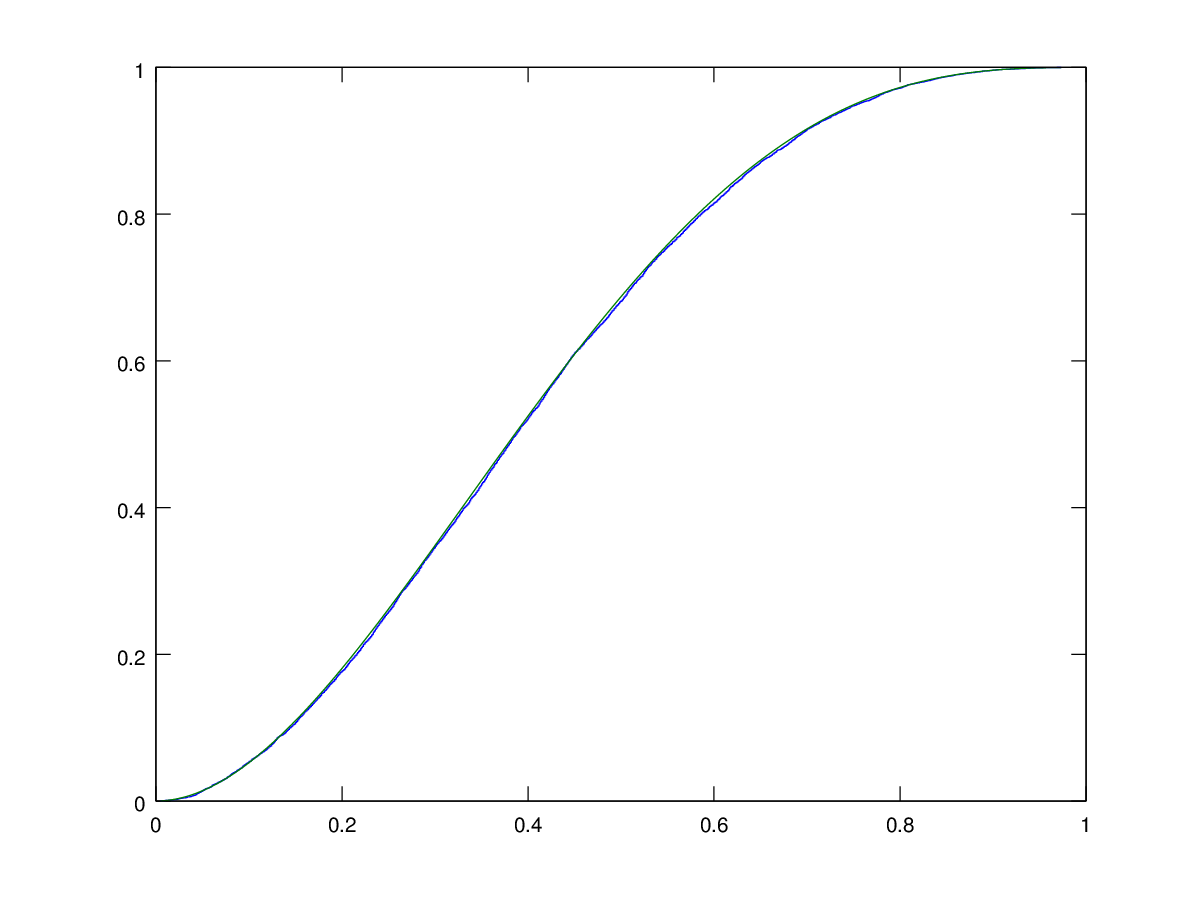
\includegraphics[width=8cm]{tarea3/problema3_4/poylaBeta.PNG}
\end{center}
\begin{center}
    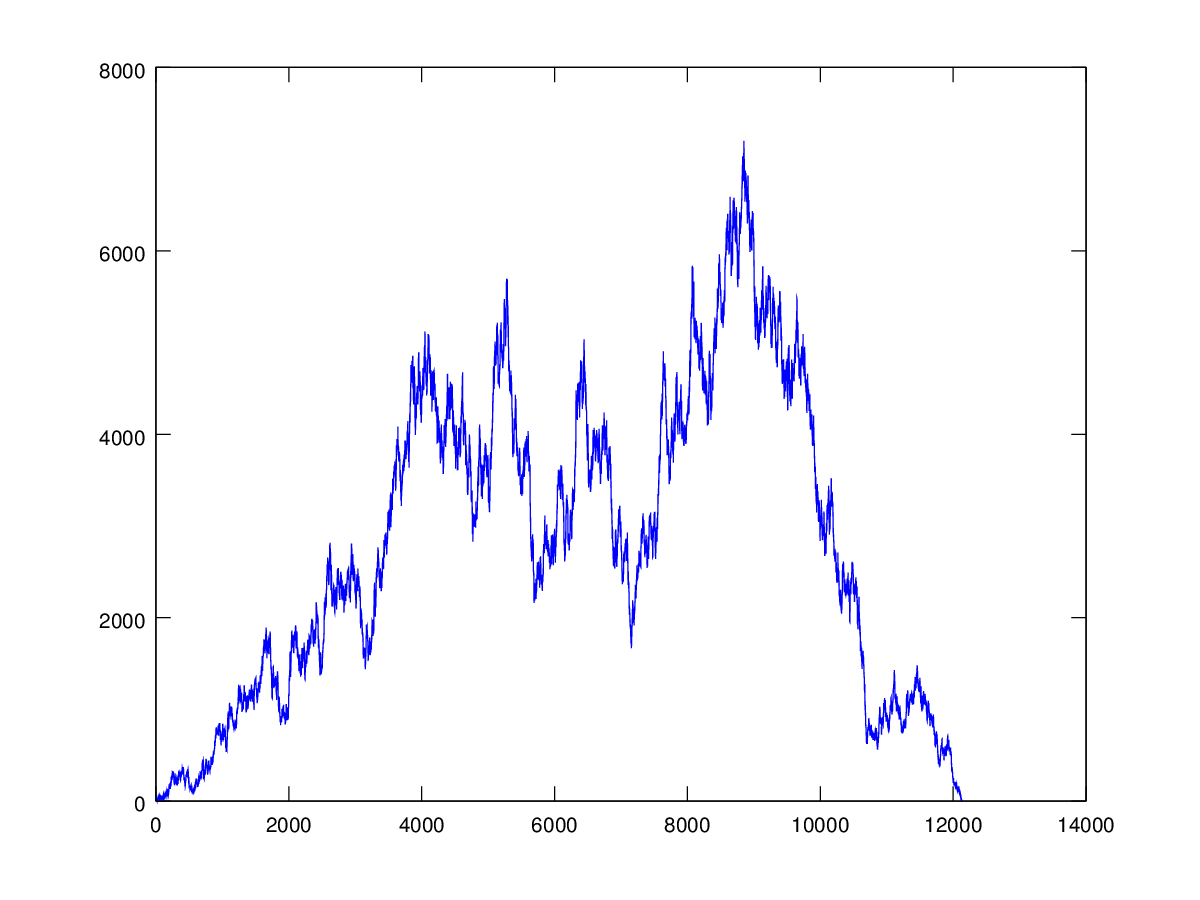
\includegraphics[width=8cm]{tarea3/problema3_4/galtonWatson.PNG}
\end{center}



